% Escreva aqui a solução da questão 6.

%\textcolor{red}{ VERSÃO 1 } %Esther

Para tanto, precisamos que a equação $ax^2 + 4x + a = 0$ não tenha solução, ou
seja, que $\Delta<0$. Segue:
\begin{align*}
    (-4)^2-4\cdot a\cdot a < 0 & \iff 16-4a^2 < 0    \\
                               & \iff 4-a^2 < 0      \\
                               & \iff  a^2-4 > 0     \\
                               & \iff (a-2)(a+2) >0.
\end{align*}
Fazendo o estudo do sinal:
\begin{center}
    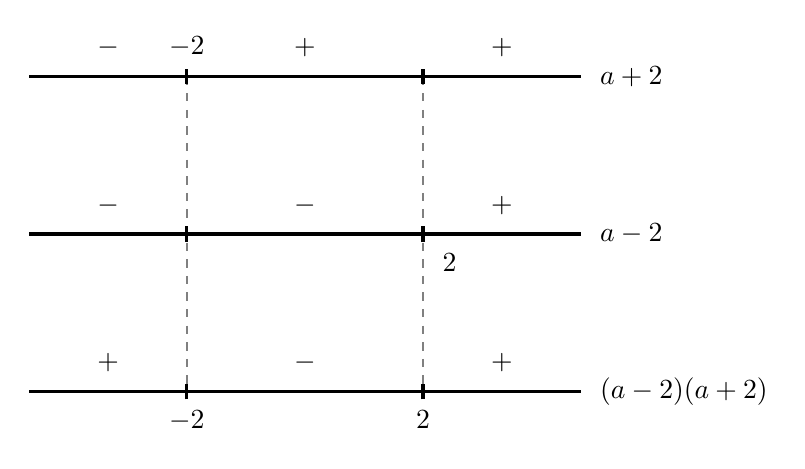
\begin{tikzpicture}
        \node[label=above:{$-2$} ] at (2,6) {};
        \node[label=south east:{2} ] at (5,4) {};
        \node[label=south:{$-2$} ] at (2,2) {};
        \node[label=south:{2} ] at (5,2) {};
        \node[label=east:{$a+2$} ] at (7,6) {};
        \node[label=east:{$a-2$} ] at (7,4) {};
        \node[label=east:{$(a-2)(a+2)$} ] at (7,2) {};
        \node[label=above:{$-$} ] at (1,6) {};
        \node[label=above:{$+$} ] at (3.5,6) {};
        \node[label=above:{$+$} ] at (6,6) {};
        \node[label=above:{$-$} ] at (1,4) {};
        \node[label=above:{$-$} ] at (3.5,4) {};
        \node[label=above:{$+$} ] at (6,4) {};
        \node[label=above:{$+$} ] at (1,2) {};
        \node[label=above:{$-$} ] at (3.5,2) {};
        \node[label=above:{$+$} ] at (6,2) {};
        \draw[very thick] (0, 6) -- (7,6);
        \draw[very thick] (0, 4) -- (7,4);
        \draw[very thick] (0, 2) -- (7,2);
        \draw[gray, thick, dashed] (2, 6) -- (2, 2);
        \draw[gray, thick, dashed] (5, 6) -- (5, 2);
        \draw[very thick] (2, 5.9) -- (2, 6.1);
        \draw[very thick] (5, 5.9) -- (5, 6.1);
        \draw[very thick] (2, 1.9) -- (2, 2.1);
        \draw[very thick] (2, 3.9) -- (2, 4.1);
        \draw[very thick] (5, 3.9) -- (5, 4.1);
        \draw[very thick] (5, 1.9) -- (5, 2.1);
    \end{tikzpicture}
\end{center}

Logo, a expressão é sempre diferente de zero quando $(a-2)(a+2) >0$, ou seja,
quando $a\in(-\infty,-2)\cup(2,+\infty)$.

\bigskip

\textcolor{red}{CHAVE DE PONTUAÇÃO:
    \begin{itemize}
        \item  Identificar que é necessário resolver $\Delta <0$ \emph{(1,0 ponto)};
        \item  Solução da inequação fazendo estudo do sinal da expressão fatorada\emph{(2,0
                  pontos)}.
    \end{itemize} }